\chapter{The GBT Observing Process}\label{chap:process}

\vspace{-0.5cm}

\section{Overview Of The Green Bank Telescope}

The 100 meter \glsfirst{GBT} is intended to address a very broad range 
of astronomical problems at radio wavelengths and consequently has an
unusual and unique design. Unlike conventional telescopes that have feed
legs projecting over the middle of the surface, the \gls{GBT}'s aperture
is unblocked so that incoming radiation meets the surface directly. This
increases the useful area of the telescope and reduces reflection and
diffraction, which ordinarily complicate a telescope's pattern of response
to the sky. To keep the aperture unblocked, the design incorporates an
off-axis feed arm that cradles the dish and projects upward at one edge.
This requires that the figure of the telescope surface be asymmetrical.
To make a projected circular aperture 100 meters in diameter, the dish is
actually a 100 by 110 meter section of a conventional, rotationally
symmetric 208 meter figure, beginning four meters outward from the
vertex of the hypothetical parent structure (see
Figure~\ref{fig:GBT}). The \gls{GBT}'s lack of circular symmetry
greatly increases the complexity of its design and construction.

\begin{figure}[!h]
\begin{center}
\subfloat[\label{fig:parentparabola}]
{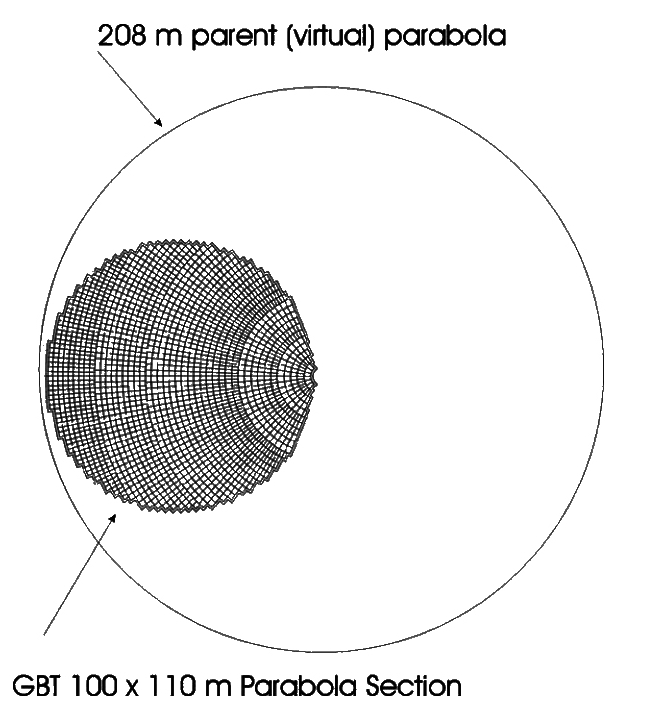
\includegraphics[width=.3\linewidth]{parent-parabola_crop.jpg}}
\hspace{.1\linewidth}
\subfloat[\label{fig:offaxis}]
{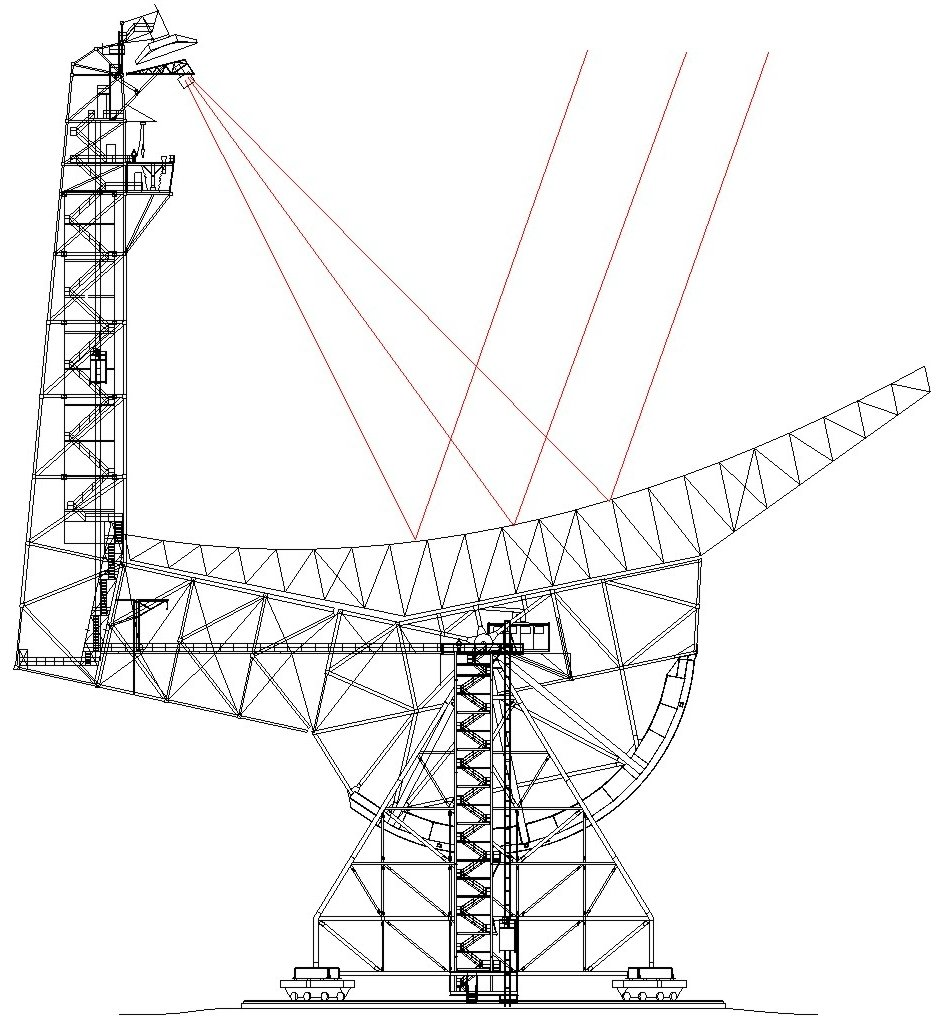
\includegraphics[width=.3\linewidth]{gbt_offaxis_crop.jpg}}
\caption[The parent parabola and off-axis design of the GBT]
{The parent parabola (\ref{fig:parentparabola}) and off-axis design
(\ref{fig:offaxis}) of the \gls{GBT}.\label{fig:GBT}}
\end{center}
\end{figure}

To maintain precise surface figures and pointing accuracy at high frequencies 
the telescope is equipped with a complex \gls{AS}. At higher frequencies
gravity distorts the surface figure of the telescope to unacceptable levels.
Temperature variations and wind can also deform the figure of the dish. To
compensate for these distortions, the surface of the \gls{GBT} is \dq{active}
i.e. it is made up of 2008 independent panels and each of these panels are
mounted on actuators at the corners, which can raise and lower the panels to
adjust the shape of the dish's surface. 

\newpage

\subsection{Main Features of the GBT}


\begin{itemize}[leftmargin=*,itemsep=1pt]
\item {\bf Fully steerable antenna}: +5$^\circ$ to +90$^\circ$ elevation range 
(-46.5$^\circ$ to +90$^\circ$ declination); 85\% coverage of the celestial sphere.  
Note that observing at elevations $>$86$^\circ$ (or 80$^\circ$ during extremely
cold weather) may fail due to the high azimuth rates required.
\item {\bf Unblocked aperture}: Reduces sidelobes, \gls{RFI}, and spectral standing waves.
\item {\bf Active surface}: Compensates for gravitational and thermal distortions.
\item {\bf Frequency coverage of 100 MHz to 115+ GHz}: 3 orders of magnitude of
frequency coverage for maximum scientific flexibility.
\item {\bf Location in the National Radio Quiet Zone}: Comparatively low \gls{RFI}
environment\\ (See Figure~\ref{fig:nrqz}).
\item {\bf Dynamic Scheduling}: Matching scientific programs to the required
weather conditions.
\end{itemize}

\glsunset{NAD83}
\glsunset{NAVD88}

\begin{table}[!h]
\begin{center}
\begin{tabular}{p{.25\linewidth}p{.6\linewidth}}
\toprule
Location & Green Bank, West Virginia, USA \\
\midrule
Coordinates & Longitude: $79\degree 50\arcminute 23.406\arcsecond$ West (\gls{NAD83})\newline
              Latitude: $38\degree 25\arcminute 59.236\arcsecond$ North (\gls{NAD83})\newline
              Track Elevation: 807.43~m (\gls{NAVD88})\\
\midrule
Optics & 110~m $\times$ 100~m unblocked section of a 208~m parent paraboloid Offaxis feed arm\\
\midrule
Telescope Diameter & 	100 m (effective) \\
\midrule
Available Foci & Prime and Gregorian \newline
                 f/D (prime) = 0.29 (referred to 208 m parent parabola) \newline
                 f/D (prime) = 0.6 (referred to 100 m effective parabola) \newline
                 f/D (Gregorian) = 1.9 (referred to 100 m effective aperture) \\
\midrule
Receiver mounts & Prime: Retractable boom with Focus-Rotation Mount \newline
                  Gregorian: Rotating turret with 8 receiver bays \\
\midrule
Subreflector & 	8-m reflector with Stewart Platform (6 degrees of freedom) \\
\midrule
Main reflector & 2004 actuated panels (2209 actuators) \newline
                 Average intra-panel RMS $68~\mu$m \\
\midrule
FWHM Beamwidth & Gregorian Feed: $\sim{ 12.60\arcminute / f_{GHz}}$ \newline
                 Prime Focus: $\sim {13.01\arcminute / f_{GHz}}$ \\
\midrule
Elevation Limits & Lower limit: $5\degree$ \newline
                   Upper limit: $90\degree$ \\
\midrule
Declination Range  & Lower limit: $-46.5\degree$ \newline
                     Upper limit: $90\degree$ \\
\midrule
Slew Rates & Azimuth:	$35.2\degree$/min \newline
             Elevation: $17.6\degree$/min \\
\midrule
Surface RMS & Passive surface: $450~\mu$m at $45\degree$ elevation,
              worse elsewhere \newline
              Active surface: $\sim250~\mu$m, under benign night-time conditions \\
\midrule
Tracking accuracy ($\sigma_{tr}$) & $\sigma_{tr}^2 = \sigma_0^2 + \left(s/3.5\right)^4$ \newline
                                   $\sigma_0$ = night:1.32\arcsecond, day:2.19\arcsecond;
                                   $s$ = wind speed (ms$^{-1}$)\\
\midrule
Pointing accuracy & 5\arcsecond\ blind pointing accuracy \\
\bottomrule
\end{tabular}
\caption{GBT Telescope Specifications.} \label{table:antenna}
\end{center}
\end{table}

\newpage

\subsection{National Radio Quiet Zone}

The \gls{NRQZ} was established by the Federal Communications Commission (FCC)
and by the Interdepartmental Radio Advisory Committee (IRAC) on November 19,
1958 to minimize possible harmful interference to the \gls{NRAO} in Green
Bank, WV and the radio receiving facilities for the United States Navy in
Sugar Grove, WV. The \gls{NRQZ} is bounded by \glsfirst{NAD83} meridians of
longitude at 78d~29m~59.0s~W and 80d~29m~59.2s~W and latitudes of
37d~30m~0.4s~N and 39d~15m~0.4s~N, and encloses a land area of
approximately 13,000 square miles near the state border between Virginia
and West Virginia.\\

\begin{itemize}
\item Further information on the \gls{NRQZ} can be obtained at\\ \vspace{-5mm}
\begin{itemize}
\item \htmladdnormallink
{https://science.nrao.edu/facilities/gbt/interference-protection/nrqz/}
{https://science.nrao.edu/facilities/gbt/interference-protection/nrqz/}
\end{itemize}
\item Information on the West Virginia State Code Chapter 37A
\dq{Radio Astronomy Zoning Act} (WVRAZ) can be found at\\ \vspace{-5mm}
\begin{itemize}
\item \htmladdnormallink
{http://www.legis.state.wv.us/WVcode/code.cfm?chap=37a\&art=1}
{http://www.legis.state.wv.us/WVcode/code.cfm?chap=37a\&art=1}
\end{itemize}
\end{itemize}

\begin{figure}[!h]
\begin{center}
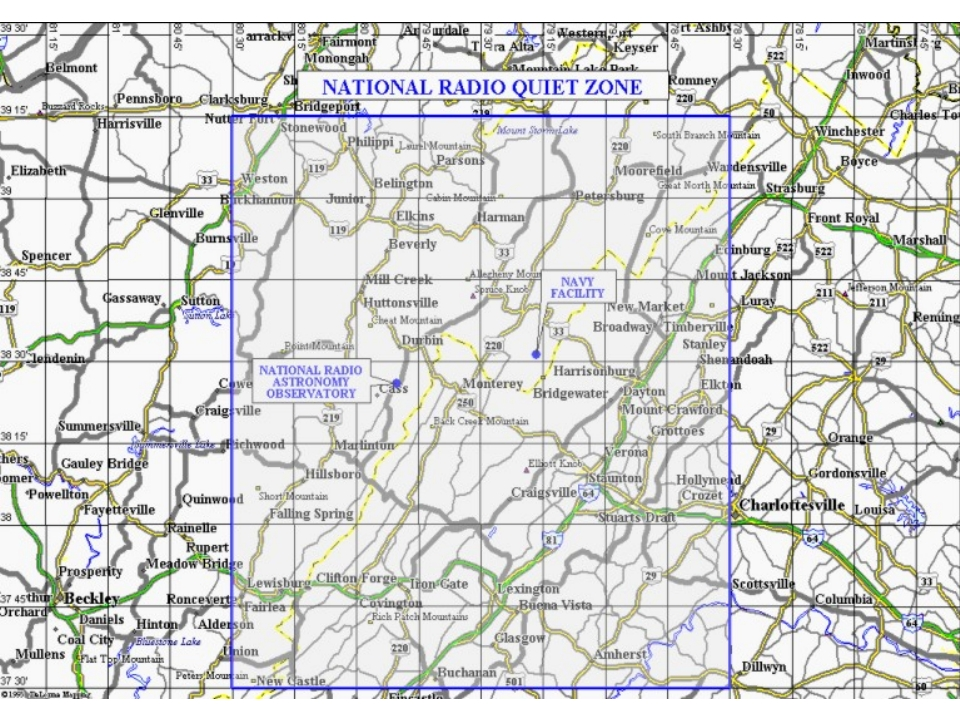
\includegraphics[width=\linewidth]{NRQZ.jpg}
\caption[National Radio Quiet Zone]
{The National Radio Quiet Zone.
\label{fig:nrqz}}
\end{center}
\end{figure}

\newpage


\subsection{Front Ends}

The \gls{GBT} receivers cover several frequency bands from
0.290 - 50 GHz and 70 - 100 GHz. Table~\ref{table:rx} lists the properties
of the Prime Focus receivers and the Gregorian Focus receivers. System temperatures
are derived from lab measurements or from expected receiver performance given
reasonable assumptions about spillover and atmospheric contributions.

The \gls{GBT} Proposer's Guide (\htmladdnormallink
{https://science.nrao.edu/facilities/gbt/proposing/GBTpg.pdf}
{https://science.nrao.edu/facilities/gbt/proposing/GBTpg.pdf}) 
provides more information on the \gls{GBT} receivers.

%\begin{table}[!h]
%\begin{center}
%\caption[Prime Focus receiver properties]{Properties of the Prime Focus 
%Receivers.}\label{table:pfrx}
%\begin{tabular}{llcccccc}
%\toprule
%\multicolumn{2}{c}{Name} & Freq. Range (GHz) & Polarization & Beams & Polns/Beam & 	\gls{Trec} & \gls{Tsys} \\
%\midrule
%\gls{PFone} & Rcvr\_342 & 0.290-0.395 &	Lin/Circ &	1 &	2 &	12 &	46 \\
%\gls{PFone} & Rcvr\_450 & 0.385-0.520 &	Lin/Circ &	1 &	2 &	22 &	43 \\
%\gls{PFone} & Rcvr\_600 & 0.510-0.690 &	Lin/Circ &	1 &	2 &	12 &	22 \\
%\gls{PFone} & Rcvr\_800 & 0.680-0.920 &	Lin/Circ &	1 &	2 &	21 &	29 \\
%\gls{PFtwo} & Rcvr\_1070& 0.910-1.230 &	Lin/Circ &	1 &	2 &	10 &	17 \\
%\bottomrule
%\end{tabular}
%\end{center}
%\end{table}

\begin{table}[!h]
\begin{center}
\caption[GBT receiver properties]
{Properties of the Prime Focus and Gregorian Focus Receivers.}
\label{table:gregrx}
\begin{tabular}{llcccccc}
\toprule
\multicolumn{2}{c}{Name} & $\nu$ Range & Polarization & Beams & Polns/& \gls{Trec} & \gls{Tsys} \\
   &                     & (GHz)       &              &       & Beam  &    (K)     &   (K)      \\
\midrule
\addlinespace
\multicolumn{8}{c}{--- Prime Focus Receivers ---}\\
\addlinespace
%\cmidrule(l{7em}r){2-5}
\gls{PFone} & Rcvr\_342 & 0.290-0.395 &	Lin/Circ &	1 &	2 &	12 &	46 \\
\gls{PFone} & Rcvr\_450 & 0.385-0.520 &	Lin/Circ &	1 &	2 &	22 &	43 \\
\gls{PFone} & Rcvr\_600 & 0.510-0.690 &	Lin/Circ &	1 &	2 &	12 &	22 \\
\gls{PFone} & Rcvr\_800 & 0.680-0.920 &	Lin/Circ &	1 &	2 &	21 &	29 \\
\gls{PFtwo} & Rcvr\_1070& 0.910-1.230 &	Lin/Circ &	1 &	2 &	10 &	17 \\
\addlinespace
\midrule
\addlinespace
\multicolumn{8}{c}{--- Gregorian Focus Receivers ---} \\
\addlinespace
\gls{Lband} & Rcvr1\_2           & 1.15-1.73 & Lin/Circ & 1 & 2 &      6 & 20 \\
\gls{Sband} & Rcvr2\_3           & 1.73-2.60 & Lin/Circ & 1 & 2 &   8-12 & 22 \\
\gls{Cband} & Rcvr4\_6           & 3.95-8.0  & Lin/Circ & 1 & 2 &     5  & 18 \\
\gls{Xband} & Rcvr8\_10          & 8.00-10.1 & Circ     & 1 & 2 &     13 & 27 \\
\gls{Kuband}& Rcvr12\_18         & 12.0-15.4 & Circ     & 2 & 2 &     14 & 30 \\ %\midrule
\gls{KFPA}  & RcvrArray18\_26    & 18.0-26.5 & Circ     & 7 & 2 &  15-25 & 30-45 \\
\gls{Kaband}& Rcvr26\_40 (MM-F1) & 26.0-31.0 & Lin      & 2 & 1 &     20 & 35 \\
\gls{Kaband}& Rcvr26\_40 (MM-F2) & 30.5-37.0 & Lin      & 2 & 1 &     20 & 30 \\
\gls{Kaband}& Rcvr26\_40 (MM-F3) & 36.0-39.5 & Lin      & 2 & 1 &     20 & 45 \\
\gls{Qband} & Rcvr40\_52         & 38.2-49.8 & Circ     & 2 & 2 &  40-70 & 67-134 \\ %\midrule
\gls{Wband} & Rcvr68\_92 (FL1)   & 67-74     & Lin/Circ & 2 & 2 & 50  & 160 \\ 
\gls{Wband} & Rcvr68\_92 (FL2)   & 73-80     & Lin/Circ & 2 & 2 & 50  & 120 \\ 
\gls{Wband} & Rcvr68\_92 (FL3)   & 79-86     & Lin/Circ & 2 & 2 & 50  & 100 \\ 
\gls{Wband} & Rcvr68\_92 (FL4)   & 85-92     & Lin/Circ & 2 & 2 & 60  & 110 \\ 
%MUSTANG & 80-100   &     -     &     64 & - &   -   & - \\
\bottomrule
\end{tabular}
\end{center}
\end{table}

\subsubsection{Prime focus receivers}

The Prime focus receivers are mounted in a \gls{FRM} on a retractable boom.
The boom is moved to the prime focus position when prime focus receivers are
to be used, and retracted when using Gregorian receivers. The \gls{FRM} holds
one receiver box at a time.  Currently there are two receiver boxes, \gls{PFone}
and \gls{PFtwo}.  A change from \gls{PFone} to \gls{PFtwo} receivers requires
a box change, taking about 4 hours and done only during scheduled maintenance days. 

The \gls{PFone} (0.29 - 0.92~GHz) receiver is divided into 4 frequency bands
within the same receiver box. The receivers are cooled \gls{FET} amplifiers.
The feeds for the lower three bands are short-backfire dipoles, and the feed
for the fourth (680-920MHz) is a corrugated feed horn with an \gls{OMT} polarization
splitter. A feed change, required to switch between bands, takes 4 hours and
must occur on a maintenance day. The \gls{PFtwo} (0.920 - 1.23~GHz) receiver 
uses a cooled \gls{FET} and a corrugated feed horn with the \gls{OMT}.

\newpage

\subsubsection{Gregorian focus receivers}

The Gregorian receivers are mounted in a rotating turret in a receiver room 
located at the Gregorian Focus of the telescope. The turret has 8 portals for 
receiver boxes. Up to 8 receivers can be kept cold and active at all times. 
Changing between any two Gregorian receivers that are installed in the turret
takes about 60-90 seconds.

%\subsubsection{The MUSTANG Receiver}
%\glsfirst{MUSTANG} is a multi-pixel bolometer array observing at 80-100 GHz
%mounted at the Gregorian focus.  It is both a receiver and the associated
%back end, and is described in Chapter~\ref{chap:mustang}. The \gls{MUSTANG}
%receiver must be used at elevations above 30\degree, due to the design of
%the cryogenics.


\subsection{Backends}\label{sec:backends}

The \gls{GBT} has two continuum backends: the \gls{DCR} and the \gls{CCB}.
The spectral line backend is \gls{VEGAS}.  Pulsar observations can be done
with \gls{GUPPI}.  There is a single dish mode for the \gls{VLBA} backend
that is available for high time--resolution observations.  Planetary radar
uses a specialized backend.

For more information on \gls{GBT} backends, please see the \dq{\gls{GBT}
Proposer's Guide} which is available at \htmladdnormallink
{http://www.gb.nrao.edu/gbtprops/man/GBTpg/GBTpg\_tf.html}
{http://www.gb.nrao.edu/gbtprops/man/GBTpg/GBTpg_tf.html}.

\subsubsection{Digital Continuum Receiver (DCR)}

The \gls{DCR} is the \gls{GBT}'s general purpose continuum backend.
It is used both for utility observations such as pointing, focus,
and beam-map calibrations, as well such as for continuum astronomical
observations including point-source on/offs, extended source mapping, etc.


\subsubsection{Caltech Continuum Backend (CCB)}

The \gls{CCB} is a sensitive, wideband backend designed exclusively for use
with the \gls{GBT} \gls{Kaband} (26-40~GHz) receiver. It provides a carefully
optimized \gls{RF} (not an \gls{IF}) detector circuits and the capability to
beam-switch the receiver rapidly to suppress instrumental gain fluctuations. 
There are 16 input ports (only 8 can be used at present with the \gls{Kaband}
receiver), hard-wired to the receiver's 2 feeds $\times$ 2 polarizations
$\times$ 4 frequency sub-bands (26-29.5 , 29.5-33.0; 33.0-36.5; and 36.5-40~GHz).
The \gls{CCB} allows the left and right noise-diodes to be controlled individually
to allow for differential or total power calibration. Unlike other \gls{GBT}
backends, the noise-diodes are either on or off for an entire integration (there
is no concept of \dq{phase within an integration}). The minimum practical
integration period is 5 milliseconds; integration periods longer than 0.1 seconds
are not recommended. The maximum practical beam-switching rate is about 4 kHz,
limited by the needed $250\mu s$ beam-switch blanking time. Switching slower
than 1 kHz is not recommended.

\subsubsection{VEGAS}

\glsfirst{VEGAS} is the spectral line backend for the \gls{GBT}. It consists of
eight independent dual polarization spectrometers (banks) that can be configured in
any one of 29 modes and can be used with any receiver except \gls{MUSTANG}. It
provides up to 64 spectral windows as well as wide bandwidths (1000-1500~MHz).
See chapter~\ref{chap:vegas} for detailed information on \gls{VEGAS}.


\subsubsection{GUPPI}

\glsfirst{GUPPI} has one hardware mode and many software modes.  \gls{GUPPI}
can be used with any receiver with the exception of \gls{MUSTANG}.  Only one
polarization would be available for the \gls{Kaband} (26-40~GHz) receiver.
\gls{GUPPI} uses 8-bit sampling to dramatically improve dynamic range and
\gls{RFI} resistance.  Currently \gls{GUPPI} can use bandwidths of 100, 200
and 800 MHz with 2 polarizations and full stokes parameters.  The minimum
integration time is $40.96\mu s$ using 2048 channels and an 800 MHz bandwidth.
See the introduction to \gls{GUPPI} in Chapter~\ref{chap:GUPPI}.


%\subsubsection{MUSTANG}
%
%See the introduction to \gls{MUSTANG} in Chapter~\ref{chap:mustang}.

\subsubsection{\dq{VLBI}}

The \gls{GBT} supports \glsfirst{VLB} observations with a Mark5 \gls{VLBA}
recorder. This recorder can also be used in a \dq{single-dish} mode to make
high time--resolution observations.  See Chapter~\ref{chap:vlba} for more
information.

\subsubsection{Radar}
Planetary radar observations are supported by the \glsfirst{PFS} and
JPL radar backends.  See Chapter~\ref{chap:radar} for more information.

\subsection{Polarization Measurements}

Measurement of Polarization and Stokes parameters is possible using
\gls{VEGAS} and \gls{GUPPI}.  This is an \dq{expert user} mode: users should
contact their GBT support person or the GBT helpdesk.  For an introduction to
polarization observations, see \dq{A Heuristic Introduction to
Radioastronomical Polarization}, by C. Heiles, ASP Conference Series
Vol 278, 2002.

\newpage

\section{The GBT Observing Process}

The following list summarizes the general flow of how \gls{GBT} observing
proceeds. By the time you are reading this document you should have already
been through several of the steps.

\begin{description}[leftmargin=*]
\item[Step 1 - Contact your GBT \dq{friend}]\ \\
Before you observe, you need to prepare for your observations
(see Chapter~\ref{chap:travel}) and set up your computing account
(see Chapter~\ref{chap:computing}). You will be assigned a scientific
contact person (\gls{GBT} \dq{friend}) whom you should contact well in
advance of your observing to determine optimum dates for a visit and ensure
the telescope and hardware will be available for the project while you are
on site. Your \dq{friend} will help you develop a appropriate observing tactics
for your proposal (see Chapter~\ref{chap:tactics}). They will also help you
with any technical questions e.g., dealing with \gls{RFI} (see
Chapter~\ref{chap:rfi}), etc. At this time you should review your project
page(s) in the \glsfirst{DSS} (see Chapter~\ref{chap:dss}) and develop your
\glsfirstplural{SB} (see Chapter~\ref{chap:scripts}).

\item [Step 2 - Make travel arrangements]\ \\
If you are an experienced \gls{GBT} observer, you can observe remotely
(see Chapter~\ref{chap:remote}). If you are new to the \gls{GBT}, you
must plan to travel to Green Bank (see Chapter~\ref{chap:travel}) and
spend at least a week and preferably two weeks at the site to ensure
appropriate weather conditions for the observations (see
Chapter~\ref{chap:weather}). You should arrive in Green Bank at least
one business day before your observations. This will allow you to meet
with the contact scientist and also with the scientific staff person who
will be \dq{on call} during your observations (these might be different people).
After hands-on experience with observing you will qualify for remote observing.

\item [Step 3 - Set blackout dates in the DSS]\ \\
If there are periods of time or dates when you cannot observe, you should
indicate these as \dq{blackout dates} in the \gls{DSS} web page
\htmladdnormallink{https://dss.gb.nrao.edu}{https://dss.gb.nrao.edu}.
Those visiting Green Bank should use blackout dates to mark the periods of
their travel before and after their stay to ensure they are scheduled only
when available and ready.

\item [Step 4 - Wait for scheduling notification]\ \\
Unless you are running a project which must be fixed to a certain date and
time, your observations will be dynamically scheduled.  See
Chapter~\ref{chap:dss} for details on how dynamical scheduling is done with
the \gls{GBT}. When your project is scheduled you will receive an e-mail
notification indicating the exact time the observing session will start.
Notifications go to the project PI and all others designated as observers
on the project.  Thus you should have prepared your scripts and be ready
to observe with 24-36 hours notice.  

\item [Step 5 - 30 minutes before your observation session]\ \\
If you are present in Green Bank, go to the control room and log into
one of the computers.  Bring up any programs that you need so that you are
prepared when your observation time begins.

If you are observing remotely (see Chapter~\ref{chap:remote}) you should
contact the \gls{GBT} operator through \textit{talk and draw}
(see~\ref{sec:talkanddraw}) or call on 304-456-2341 or 304-456-2346.  In case
of a site phone or power outage, the direct line to the control room is
304-456-3203. You should give the operator your contact information (phone
numbers, emails) so that they can contact you during the observations
if necessary.  You will also need to let the operator know what computer
you will be using during your observations.  At this time you will begin
to open a \gls{VNC} session that you will use for the remote observations.
Starting this early will allow for any problems encountered while preparing
to observe remotely to be solved before the observations are to begin.
\vspace{-5mm}
\begin{itemize}[leftmargin=*,itemsep=0pt]
\item You can find information about \gls{GBT} remote observing policies at\\
\vspace{-5mm}
\begin{itemize}[itemsep=0pt]
\item \htmladdnormallink
{https://science.nrao.edu/facilities/gbt/observing/policies}
{https://science.nrao.edu/facilities/gbt/observing/policies}
\end{itemize}
\item You can find information about opening a \gls{VNC} session at\\
\vspace{-5mm}
\begin{itemize}[itemsep=0pt]
\item \htmladdnormallink
{https://science.nrao.edu/facilities/gbt/observing/remote-observing-with-the-gbt}
{https://science.nrao.edu/facilities/gbt/observing/remote-observing-with-the-gbt}.
\end{itemize}
\end{itemize}

\newpage

\item [Step 6 - Operator responsibilities]\ \\
The operator on duty will handle several tasks for you at the beginning of
your observations.  They will \dq{put you in the gateway} (give you security
access) so that you can control the \gls{GBT}.  They will also get the correct
receiver into the focus position of the \gls{GBT}, get the antenna motor drives
ready for movement, place the correct pointing models into the system, and set
the \gls{GBT}'s \glsfirst{AS} into the proper state.  The operator is there
to take care of all safety issues concerning the \gls{GBT}.

\item [Step 7 - Begin observations]\ \\
Now you are ready to observe.  You will use the \gls{Astrid} (see
Chapter~\ref{chap:astrid}) to perform your observations by submitting an
\gls{SB} (see Chapter~\ref{chap:scripts}).  The steps you will take in
observing are generally:
\begin{enumerate}[leftmargin=*,label={\bf \Alph*}]
\item Configure the hardware to the desired states. The parameters used
to determine these states are known as the \dq{configuration} and the
act of setting these states is known as \dq{configuring}.
\item Slew to your source.
\item Balance the \gls{IFsys}. In this step you command the system to
automatically adjust amplifier and attenuator settings in the \gls{IFsys} to
ensure that all components operate within their linear regime.
\item Execute your observations using one of the \gls{SB} Scan Types
(see Chapter~\ref{chap:scripts}).
\item If problems develop let the operator know and they will either help
solve the issue or contact the on-call support scientist for assistance. 
\end{enumerate}

\item [Step 8 - Immediately after observations]\ \\
Once you are done observing you should close \gls{Astrid}, log out of
the computer you were using, and leave the control room.  Or, if
observing remotely, {\bf properly close your \gls{VNC} session} using the
{\tt vncserver -kill} command.

\item [Step 9 - Data reduction]\ \\
During and after your observing run you will reduce your data. You will generally
use \gls{GBTIDL} for data reduction of spectral line data.  This can be done
either at Green Bank or your home institution.  Continuum reduction support is
available for the \gls{CCB} (see Chapter~\ref{chap:ccb}).  Otherwise only rudimentary continuum data reduction
support is available for the \gls{GBT} at this time, and you should contact
your \gls{GBT} \dq{friend} for more information. A pulsar data reduction
package, \glsunset{PRESTO}\gls{PRESTO}, is available from Scott Ransom.

Use one of the data reduction machines, not the workstations used for running
the observations.  Refer to \htmladdnormallink
{http://www.gb.nrao.edu/pubcomputing/data-reduction.shtml}
{http://www.gb.nrao.edu/pubcomputing/data-reduction.shtml}
for a list of data reduction machines at Green Bank.

Note that observers wishing to reduce VEGAS data will need access to the
\dq{lustre} file system.  Refer to
\htmladdnormallink{http://www.gb.nrao.edu/pubcomputing/public.shtml}
{http://www.gb.nrao.edu/pubcomputing/public.shtml} for a list of lustre clients.

\item [Step 10 - Transfer your data]\ \\
Once you are done you will want to transfer your data to your home institution
(see Chapter~\ref{chap:after}).

\item [Step 11 - Keep in touch]\ \\
Finally you will want to write your Nobel Prize winning paper. The \gls{NRAO} can
help you with your page charges (see Chapter~\ref{chap:after}). You should also
notify your scientific contact person of your paper to help the Observatory
keep track of how successful all observing projects have been.

\end{description}



%%%%%%%%%% END CHAPTER....